\documentclass{article}
\PassOptionsToPackage{quiet}{fontspec}
\usepackage[UTF8]{ctex}
\usepackage{amsmath,amssymb}
\usepackage{braket}
\usepackage{enumitem}
\usepackage{graphicx}
\usepackage{float} 
\usepackage{geometry}
\geometry{top=2cm, bottom=2cm, textwidth=16cm}
\title{HHL算法详细求解过程}
\author{王心锐}

\begin{document}
\maketitle

\section{概述}
HHL算法用于求解线性方程组 \( A\vec{x} = \vec{b} \),其中 \( A \) 为 \( N_b \times N_b \) 厄米矩阵,
\(\vec{x}\)和\(\vec{b}\)为\( N_b \)维向量,其解可表示为\( \vec{x} = A^{-1}\vec{b} \),其中\( N_b=2^{n_b} \)。
该算法通过量子态的振幅编码和演化,实现了相比经典方法的指数级加速,是量子计算中解决线性系统问题的核心算法之一。

算法中向量 \(\vec{b}\) 和 \(\vec{x}\) 的 \(N_b\) 个分量通过振幅编码(amplitude encoding),由 \(n_b\) 个量子比特(构成 \(\mathbb{C}^{N_b}\) 希尔伯特空间,记为 b-register )进行编码,\(n_b\) 需足够大以完整编码 \(\vec{b}\) 。矩阵 \(A\) 则通过哈密顿量编码(Hamiltonian encoding)模拟实现。

HHL 算法主要包含五大核心模块:状态制备(state preparation)、量子相位估计(quantum phase estimation, QPE)、辅助比特旋转(ancilla bit rotation)、逆量子相位估计(inverse quantum phase estimation, IQPE)及测量(measurement) 。
除 \(n_b\) 个用于编码 \(\vec{b}\) 振幅及最终存储 \(\vec{x}\) 结果振幅的量子比特外,算法还需 1 个辅助量子比特 \(|\rangle_a\) 与 \(n\) 个时钟量子比特(clock qubits,记为 c-register )。辅助量子比特虽最终会被舍弃,但对算法目标实现至关重要;时钟量子比特用于存储矩阵 \(A\) 编码后的特征值,且 \(n\) 越大(对应 \(N = 2^n\) ),在编码非精确场景下算法结果精度越高 。 

作为哈密顿量的矩阵 \(A\),可在其本征向量基下展开为线性组合形式。由于 \(A\) 是哈密顿量,它可表示为其本征向量 \(|u_i\rangle\) 按本征值 \(\lambda_i\) 加权的线性组合,即:
\[A = \sum_{i=0}^{2^{n_b}-1} \lambda_i |u_i\rangle \langle u_i|\]
其中,\(n_b\) 为与编码相关的量子比特数,对应构建的希尔伯特空间维度为\(2^{n_b}\)。
鉴于 \(A\) 在其本征向量基下是对角矩阵,其逆矩阵 \(A^{-1}\) 可简便表示为:
\[A^{-1} = \sum_{i=0}^{2^{n_b}-1} \lambda_i^{-1} |u_i\rangle \langle u_i|\]
同时,向量 \(\vec{b}\) 也能在 \(A\) 的本征向量基下展开,形式为:
\[|b\rangle = \sum_{j=0}^{2^{n_b}-1} b_j |u_j\rangle\]

基于上述展开,结合 \(\langle u_i|u_j\rangle = \delta_{ij}\)(\(\delta_{ij}\) 为克罗内克函数,\(i = j\) 时为 1,否则为 0 )这一性质,原线性方程组可编码为量子态形式。最终,解 \(|x\rangle\) 满足:
\[|x\rangle = A^{-1} |b\rangle = \sum_{i=0}^{2^{n_b}-1} \lambda_i^{-1} b_i |u_i\rangle\]
HHL 算法的目标便是以这种形式求解,且解 \(|x\rangle\) 存储于 b-register 中 。

\begin{figure}[htbp]
    \centering
    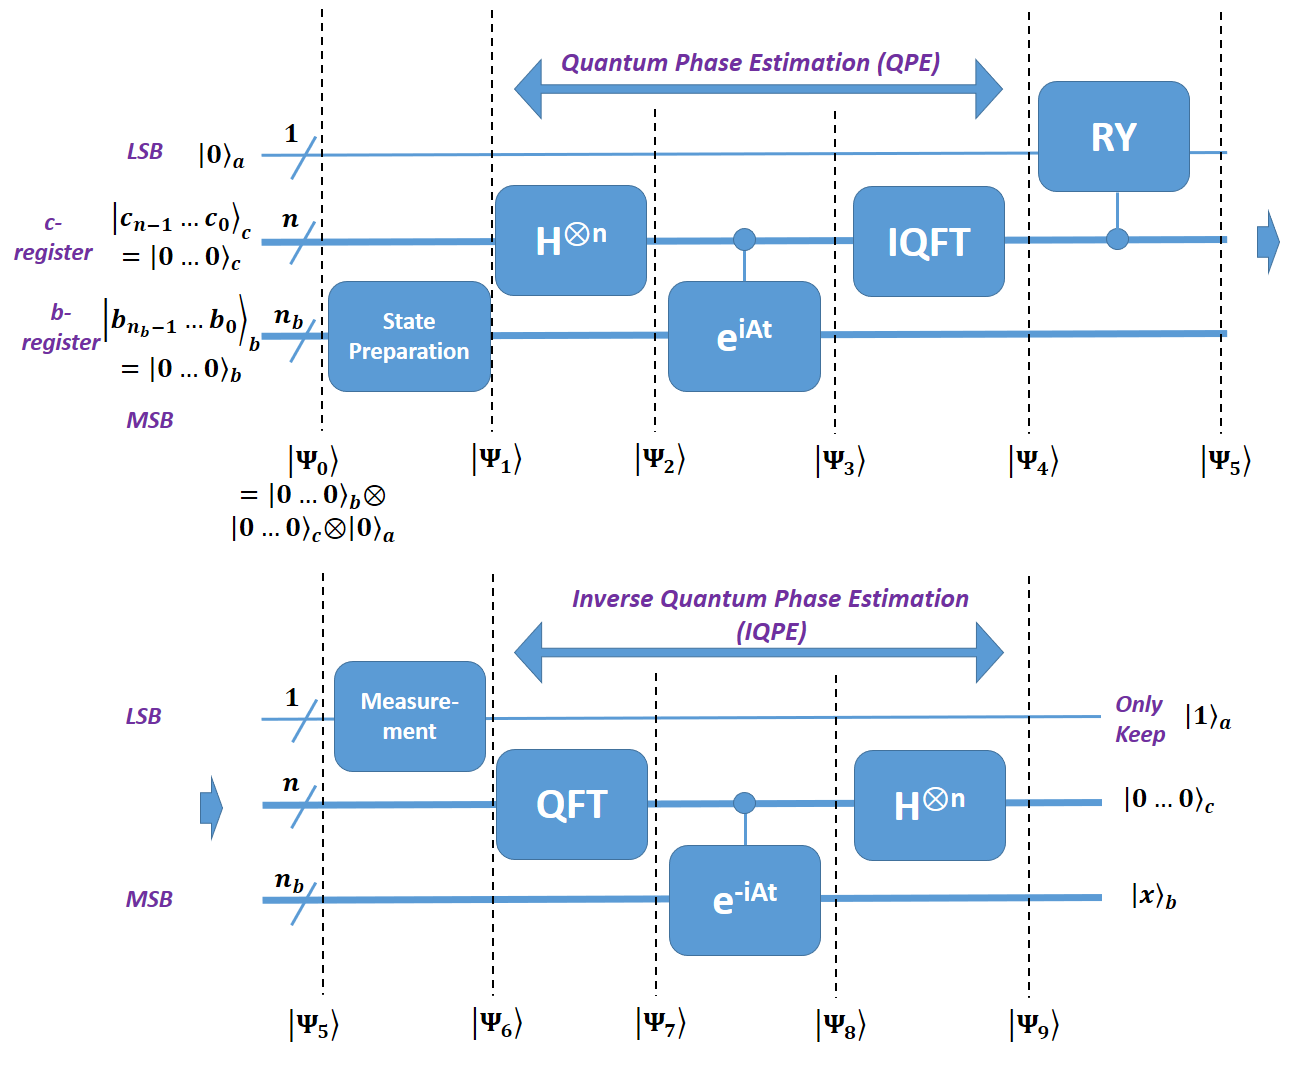
\includegraphics[width=0.7\textwidth]{/home/wangxinrui/Quantum-Computing/HHL1.png}
    \caption{HHL量子电路从左到右的结构示意图。根据小端字序约定,图中最低的量子位是最高有效位(MSB),而最上方的则是最低有效位(LSB)。}
\end{figure}
\section{算法核心步骤}
\subsection{状态制备}
初始时,系统包含\( n_b + n + 1 \)个量子比特(\( n_b \)个用于编码向量的b寄存器、\( n \)个时钟量子比特的c寄存器、1个辅助量子比特),初始状态为:

\[\ket{\Psi_0} 
= \ket{0 \cdots 0}_b \, \ket{0 \cdots 0}_c \, \ket{0}_a 
= \ket{0}^{\otimes n_b} \, \ket{0}^{\otimes n} \, \ket{0}\]

在状态制备过程中,b-寄存器中的 \(\ket{0 \cdots 0}_b\) 需要通过旋转操作,使其振幅与向量 \(\vec{b}\) 的系数一一对应。

\[
\vec{b} 
= \begin{pmatrix} 
\beta_0 \\ 
\beta_1 \\ 
\vdots \\ 
\beta_{N_b - 1} 
\end{pmatrix} 
\quad\Leftrightarrow\quad 
\beta_0\ket{0} + \beta_1\ket{1} + \cdots + \beta_{N_b - 1}\ket{N_b - 1} 
= \ket{b}= \sum_{j=0}^{N_b-1} \beta_j \ket{j}
\]

左侧的 \(\vec{b}\) 以列向量形式呈现,其中 \(\beta_i\) 是列向量的系数,这也是量子态 \(\ket{b}\) 的有效表示;右侧则显式写出了由 \( n_b \) 个量子比特张成的希尔伯特空间的对应基矢展开形式。因此,状态制备完成后,系统量子态演化为:
\[
\ket{\Psi_1} 
= \ket{b}_b \, \ket{0 \cdots 0}_c \, \ket{0}_a = \ket{b} \otimes \ket{0}^{\otimes n} \otimes \ket{0}_a \quad \text{}
\]
\subsection{量子相位估计(QPE)}
量子相位估计(QPE)也是一种特征值估计算法。QPE包含三个部分,即通过哈达玛门实现时钟量子比特的叠加、受控旋转以及逆量子傅里叶变换(IQFT)。
\subsubsection{时钟量子比特叠加}
在创建时钟量子比特叠加的第一步中,对时钟量子比特应用哈达玛门,得到:
\[
\left|\Psi_{2}\right>=I^{\otimes n_{b}} \otimes H^{\otimes n} \otimes I\left|\Psi_{1}\right>
\]
\[
=|b\rangle \frac{1}{2^{\frac{n}{2}}}{\left(|0\rangle+|1\rangle\right)}^{\otimes n}|0\rangle
\]
\subsubsection{受控旋转}
在受控旋转部分,将$U$应用于$|b\rangle$,其中时钟量子比特作为控制量子比特(图2)。为简单起见,我们首先假设$|b\rangle$是$U$的特征向量,其特征值为$e^{2 \pi i \phi}$。因此:
\[
U|b\rangle=e^{2 \pi i \phi}|b\rangle \quad
\]
\begin{figure}[htbp]
    \centering
    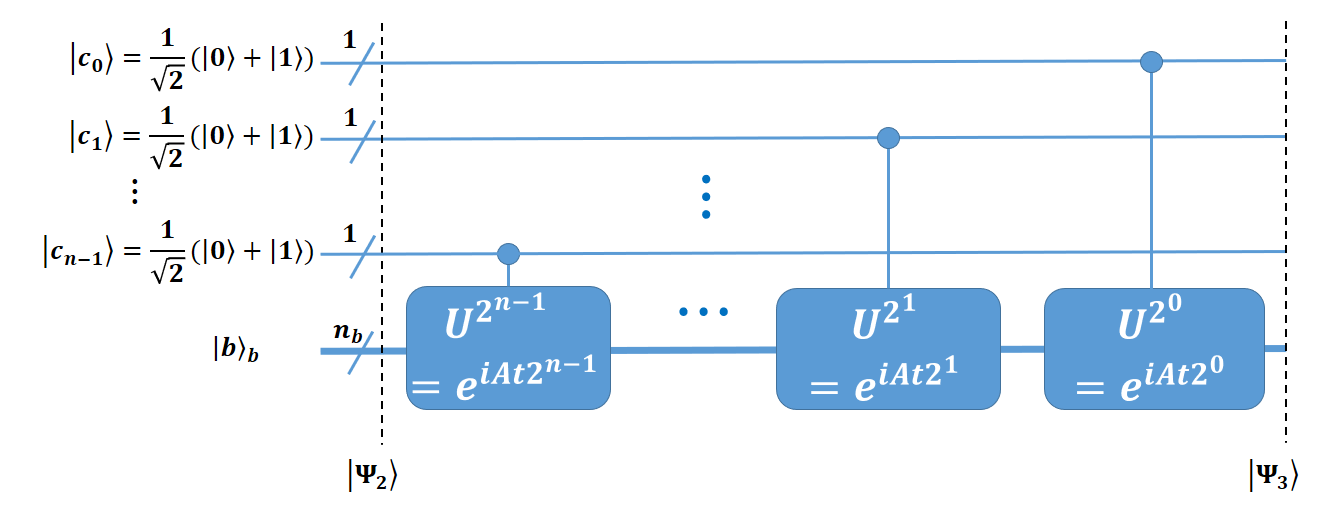
\includegraphics[width=\textwidth]{/home/wangxinrui/Quantum-Computing/HHL2.png}
    \caption{QPE 的受控旋转部分。在 HHL 算法中,$U$ 由 $e^{iAt}$ 取代。}
\end{figure}
当控制时钟量子比特为$0$时,$|b\rangle$不会受到影响。如果时钟比特为$1$,则将$U$应用于$|b\rangle$。这相当于在第$j$个时钟量子比特的$1$前面乘以$e^{2 \pi i \phi 2^{j}}$。因此,在受控$U$操作之后,我们有:
\[\begin{aligned} 
\left|\Psi_{3}\right> & =|b\rangle \otimes\left(\frac{1}{2^{\frac{n}{2}}}\left(|0\rangle+e^{2 \pi i \phi 2^{n-1}}|1\rangle\right)\otimes \cdots \otimes\left(|0\rangle+e^{2 \pi i \phi 2^{0}}|1\rangle\right)\right) \otimes|0\rangle_{a} \\ 
& =|b\rangle \frac{1}{2^{\frac{n}{2}}} \sum_{k=0}^{2^{n}-1} e^{2 \pi i \phi k}|k\rangle|0\rangle_{a} 
\end{aligned}\]
\subsubsection{逆量子傅里叶变换(IQFT)}
在IQFT部分,只有时钟量子比特受到影响。注意,在某些文献中,这被称为量子傅里叶变换(QFT)。
\[
\begin{aligned} 
\left|\Psi_{4}\right> & =|b\rangle I Q F T\left(\frac{1}{2^{\frac{n}{2}}} \sum_{k=0}^{2^{n}-1} e^{2 \pi i \phi k}|k\rangle\right)|0\rangle_{a} \\ 
& =|b\rangle \frac{1}{2^{\frac{n}{2}}} \sum_{k=0}^{2^{n}-1} e^{2 \pi i \phi k}(I Q F T|k\rangle)|0\rangle_{a} \\ 
& =|b\rangle \frac{1}{2^{n}} \sum_{k=0}^{2^{n}-1} e^{2 \pi i \phi k}\left(\sum_{y=0}^{2^{n}-1} e^{-2 \pi i y k / N}|y\rangle\right)|0\rangle_{a} \\ 
& =\frac{1}{2^{n}}|b\rangle \sum_{y=0}^{2^{n}-1} \sum_{k=0}^{2^{n}-1} e^{2 \pi i k(\phi-y / N)}|y\rangle|0\rangle_{a} 
\end{aligned}
\]

由于干涉,只有满足$\phi - y/N=0$的$|y\rangle$会有$\sum_{k=0}^{2^{n}-1} e^{0}=2^{n}$的有限振幅。否则,由于相消干涉,振幅为$\sum_{k=0}^{2^{n}-1} e^{2 \pi i k(\phi - y/N)}=0$。忽略振幅为零的状态,我们可以将$|\Psi_{4}\rangle$重写为:
\[
\left|\Psi_{4}\right>=|b\rangle|N \phi\rangle|0\rangle_{a} \quad
\]

因此,在QPE中,时钟量子比特用于表示$U$的相位信息$\phi$,其精度取决于量子比特的数量$n$。

在哈密顿量编码中,$U$与$A$的关系为:
\[
U=e^{i A t} \quad
\]

其中$t$是该哈密顿量的演化时间。显然,$U$在$A$的特征向量$|u_{i}\rangle$基下是对角的。

如果$|b\rangle = |u_{j}\rangle$,则:
\[
U|b\rangle=e^{i \lambda_{j} t}\left|u_{j}\right\rangle
\]

通过将式$U|b\rangle=e^{2 \pi i \phi}|b\rangle$中的$2\pi i\phi$等同于$i\lambda_{j}t$,我们得到$\phi=\lambda_{j}t/(2\pi)$,则$\left|\Psi_{4}\right>$变为:
\[
\left|\Psi_{4}\right>=\left|u_{j}\right\rangle\left|N \lambda_{j} t / 2 \pi\right\rangle|0\rangle_{a}
\]

这样,$A$的特征值就被编码到了时钟量子比特中(基编码)。

然而,一般来说,$|b\rangle=\sum_{j=0}^{2^{n_{b}-1}}b_{j}|u_{j}\rangle$,利用叠加原理,有:
\[
\left|\Psi_{4}\right>=\sum_{j=0}^{2^{n_{b}-1}} b_{j}\left|u_{j}\right\rangle\left|N \lambda_{j} t / 2 \pi\right\rangle|0\rangle_{a}
\]

$\lambda_{j}$通常不是整数。我们会选择$t$,使得$\tilde{\lambda_{j}}=N\lambda_{j}t/(2\pi)$为整数。因此,编码值$\tilde{\lambda_{j}}$可以与$\lambda_{j}$不同。$\Psi_{4}$可以重写为:
\[
\left|\Psi_{4}\right>=\sum_{j=0}^{2^{n_{b}-1}} b_{j}\left|u_{j}\right\rangle\left|\tilde{\lambda}_{j}\right\rangle|0\rangle_{a}
\]
\subsection{辅助量子比特的受控旋转与测量}

下一步是基于时钟寄存器(c-register)中编码的特征值旋转辅助量子比特\(|0\rangle_a\),旋转后的态为:

\[
|\Psi_5\rangle = \sum_{j=0}^{2^{n_b}-1} b_j |u_j\rangle |\tilde{\lambda}_j\rangle \left( \sqrt{1 - \frac{C^2}{\tilde{\lambda}_j^2}} |0\rangle_a + \frac{C}{\tilde{\lambda}_j} |1\rangle_a \right)
\]

其中\(C\)为常数。对辅助量子比特进行测量时,其波函数会坍缩到\(|0\rangle\)或\(|1\rangle\)。若坍缩到\(|0\rangle\),则结果会被丢弃,需重复计算直至测量结果为\(|1\rangle\)。因此,我们关注的最终波函数为:

\[
|\Psi_6\rangle = \frac{1}{\sqrt{\sum_{j=0}^{2^{n_b}-1} \left| \frac{b_j C}{\tilde{\lambda}_j} \right|^2}} \sum_{j=0}^{2^{n_b}-1} b_j |u_j\rangle |\tilde{\lambda}_j\rangle \frac{C}{\tilde{\lambda}_j} |1\rangle_a
\]

式中的归一化因子源于测量后的归一化处理。由于\(\left| \frac{C}{\tilde{\lambda}_j} \right|^2\)是测量到\(|1\rangle\)的概率,因此\(C\)应尽可能取大值。与式\(|x\rangle = A^{-1} |b\rangle = \sum_{i=0}^{2^{n_b}-1} \lambda_i^{-1} b_i |u_i\rangle\)对比可知,上述结果与目标解\(|x\rangle\)类似,但它与时钟寄存器\(|\tilde{\lambda}_j\rangle\)存在纠缠,即无法将结果分解为时钟寄存器与b寄存器的张量积。因此,我们需要通过反计算(uncomputation)来消除这种纠缠。

测量通常可在反计算后进行,但由于辅助量子比特在受控旋转后不再参与任何操作,因此在反计算前测量辅助量子比特会得到相同的结果。为简化推导,此处选择在反计算前进行测量。


\subsection{反计算——逆量子相位估计(IQPE)}

首先,对时钟寄存器应用量子傅里叶变换(QFT):

\[
\begin{aligned}
|\Psi_7\rangle &= \frac{1}{\sqrt{\sum_{j=0}^{2^{n_b}-1} \left| \frac{b_j C}{\tilde{\lambda}_j} \right|^2}} \sum_{j=0}^{2^{n_b}-1} \frac{b_j C}{\tilde{\lambda}_j} |u_j\rangle \, \text{QFT} \, |\tilde{\lambda}_j\rangle |1\rangle_a \\
&= \frac{1}{\sqrt{\sum_{j=0}^{2^{n_b}-1} \left| \frac{b_j C}{\tilde{\lambda}_j} \right|^2}} \sum_{j=0}^{2^{n_b}-1} \frac{b_j C}{\tilde{\lambda}_j} |u_j\rangle \left( \frac{1}{2^{n/2}} \sum_{y=0}^{2^n - 1} e^{2\pi i y \tilde{\lambda}_j / N} |y\rangle \right) |1\rangle_a
\end{aligned}
\]

随后,通过时钟寄存器对b寄存器应用逆受控旋转,其中\(U^{-1} = e^{-iAt}\)。与正向过程类似,当时钟量子比特为\(0\)时,\(|u_j\rangle\)不受影响;当时钟量子比特为\(1\)时,\(U^{-1}\)会作用于\(|u_j\rangle\),这等价于在第\(i\)个时钟比特的\(|1\rangle\)前乘以\(e^{-i\lambda_j t 2^i}\)。因此:

\[
|\Psi_8\rangle = \frac{1}{2^{n/2} \sqrt{\sum_{j=0}^{2^{n_b}-1} \left| \frac{b_j C}{\tilde{\lambda}_j} \right|^2}} \sum_{j=0}^{2^{n_b}-1} \frac{b_j C}{\tilde{\lambda}_j} |u_j\rangle \left( \sum_{y=0}^{2^n - 1} e^{-i\lambda_j t y} e^{2\pi i y \tilde{\lambda}_j / N} |y\rangle \right) |1\rangle_a
\]

由于我们已设置\(\tilde{\lambda}_j = N \lambda_j t / 2\pi\),因此两个指数项会相互抵消:

\[
\begin{aligned}
|\Psi_8\rangle &= \frac{1}{2^{n/2} \sqrt{\sum_{j=0}^{2^{n_b}-1} \left| \frac{b_j C}{\tilde{\lambda}_j} \right|^2}} \sum_{j=0}^{2^{n_b}-1} \frac{b_j C}{\tilde{\lambda}_j} |u_j\rangle \sum_{y=0}^{2^n - 1} |y\rangle |1\rangle_a \\
&= \frac{C}{2^{n/2} \sqrt{\sum_{j=0}^{2^{n_b}-1} \left| \frac{b_j C}{\lambda_j} \right|^2}} |x\rangle \sum_{y=0}^{2^n - 1} |y\rangle |1\rangle_a
\end{aligned}
\]

此时,时钟寄存器与b寄存器已解纠缠,且b寄存器中存储了\(|x\rangle\)。最后,对时钟寄存器应用Hadamard门。
对于多比特 \( H^{\otimes n} \)(\( n \) 个 \( H \) 门的张量积 ),其厄米共轭满足:
\({H^{\otimes n}}^\dagger = {H^\dagger}^{\otimes n} = H^{\otimes n}\)
且多比特幺正性为:
\({H^{\otimes n}}^\dagger {H^{\otimes n}} = I^{\otimes n}\)这保证了多比特态经过 \( H^{\otimes n} \) 操作后,内积运算仍满足正交性和归一性。

\[
\begin{aligned}
|\Psi_9\rangle &= \frac{1}{\sqrt{\sum_{j=0}^{2^{n_b}-1} \left| \frac{b_j C}{\lambda_j} \right|^2}} \sum_{j=0}^{2^{n_b}-1} \frac{b_j C}{\lambda_j} |u_j\rangle |0\rangle^{\otimes n} |1\rangle_a \\
&= \frac{1}{\sqrt{\sum_{j=0}^{2^{n_b}-1} \left| \frac{b_j}{\lambda_j} \right|^2}} |x\rangle_b |0\rangle_c^{\otimes n} |1\rangle_a
\end{aligned}
\]



\subsection{H门作用于多比特全0寄存器的计算过程}

\subsubsection{单比特情况}

首先考虑单比特情况,H门的定义为:
\[
H|0\rangle = \frac{|0\rangle + |1\rangle}{\sqrt{2}}
\]
\[
H|1\rangle = \frac{|0\rangle - |1\rangle}{\sqrt{2}}
\]

当H门作用于$|0\rangle$时:
\[
H|0\rangle = \frac{|0\rangle + |1\rangle}{\sqrt{2}}
\]

再将H门作用于上述结果:
\[
H\left(H|0\rangle\right) = H\left(\frac{|0\rangle + |1\rangle}{\sqrt{2}}\right)
\]
\[
= \frac{1}{\sqrt{2}}\left(H|0\rangle + H|1\rangle\right)
\]
\[
= \frac{1}{\sqrt{2}}\left(\frac{|0\rangle + |1\rangle}{\sqrt{2}} + \frac{|0\rangle - |1\rangle}{\sqrt{2}}\right)
\]
\[
= \frac{1}{\sqrt{2}} \cdot \frac{2|0\rangle}{2} = |0\rangle
\]

可见,对单比特$|0\rangle$连续作用两次H门,结果回到$|0\rangle$。

\subsubsection{多比特情况}

考虑$n$个比特的全0寄存器:
\[
|0\rangle^{\otimes n} = |0\rangle \otimes |0\rangle \otimes \cdots \otimes |0\rangle \quad (n \text{次张量积})
\]

多比特H门操作为单比特H门的张量积:
\[
H^{\otimes n} = H \otimes H \otimes \cdots \otimes H \quad (n \text{次张量积})
\]

第一次应用$H^{\otimes n}$:
\[
H^{\otimes n}|0\rangle^{\otimes n} = (H \otimes H \otimes \cdots \otimes H)(|0\rangle \otimes |0\rangle \otimes \cdots \otimes |0\rangle)
\]
\[
= H|0\rangle \otimes H|0\rangle \otimes \cdots \otimes H|0\rangle
\]
\[
= \left(\frac{|0\rangle + |1\rangle}{\sqrt{2}}\right) \otimes \left(\frac{|0\rangle + |1\rangle}{\sqrt{2}}\right) \otimes \cdots \otimes \left(\frac{|0\rangle + |1\rangle}{\sqrt{2}}\right)
\]
\[
= \frac{1}{2^{n/2}} \sum_{x=0}^{2^{n}-1} |x\rangle
\]

其中$|x\rangle$表示所有可能的$n$比特态,这是一个均匀叠加态。

第二次应用$H^{\otimes n}$:
\[
H^{\otimes n}\left(H^{\otimes n}|0\rangle^{\otimes n}\right) = H^{\otimes n}\left(\frac{1}{2^{n/2}} \sum_{x=0}^{2^{n}-1} |x\rangle\right)
\]
\[
= \frac{1}{2^{n/2}} \sum_{x=0}^{2^{n}-1} H^{\otimes n}|x\rangle
\]

对于任意$n$比特态$|x\rangle = |x_1x_2\cdots x_n\rangle$,其中$x_i \in \{0,1\}$,有:
\[
H^{\otimes n}|x\rangle = \bigotimes_{i=1}^{n} H|x_i\rangle
\]

当$x_i = 0$时,$H|0\rangle = \frac{|0\rangle + |1\rangle}{\sqrt{2}}$;当$x_i = 1$时,$H|1\rangle = \frac{|0\rangle - |1\rangle}{\sqrt{2}}$。

将这些代入求和式,展开后大部分项会相互抵消,最终结果为:
\[
H^{\otimes n_b}\left(H^{\otimes n}|0\rangle^{\otimes n}\right) = |0\rangle^{\otimes n}
\]

\subsubsection{结论}

对$n_b$比特全0寄存器连续应用两次$H^{\otimes n}$门,系统会回到初始的全0态:
\[
H^{\otimes n} \cdot H^{\otimes n} \cdot |0\rangle^{\otimes n} = |0\rangle^{\otimes n}
\]

这表明 \(H^{\otimes n}\) 是自逆的,即${{\left( H^{\otimes n} \right)}^2} = I^{\otimes n}$,其中\(I^{\otimes n}\) 是$n$比特的单位操作。





\section{数值示例}

我们将通过一个数值示例,逐步应用HHL算法。首先,我们将讨论如何实现受控-U操作和辅助量子位的旋转。

\subsection{编码方案}

在本示例中,矩阵\(A\)和向量\(\vec{b}\)设定为:
\[
A = \begin{pmatrix} 1 & -\frac{1}{3} \\ -\frac{1}{3} & 1 \end{pmatrix}
\]
\[
\vec{b} = \begin{pmatrix} 0 \\ 1 \end{pmatrix}
\]

矩阵\(A\)的特征向量为\(\vec{u}_0 = \begin{pmatrix} \frac{-1}{\sqrt{2}} \\ \frac{-1}{\sqrt{2}} \end{pmatrix}\)和\(\vec{u}_1 = \begin{pmatrix} \frac{-1}{\sqrt{2}} \\ \frac{1}{\sqrt{2}} \end{pmatrix}\),对应的特征值分别为\(\lambda_0 = \frac{2}{3}\)和\(\lambda_1 = \frac{4}{3}\)。我们需要通过基编码将特征值编码到时钟量子比特形成的基中,且需要2个量子比特:将\(\lambda_0\)编码为\(|01\rangle\),将\(\lambda_1\)编码为\(|10\rangle\),以保持\(\lambda_1/\lambda_0 = 2\)的比例。这意味着\(\tilde{\lambda}_0 = 1\)、\(\tilde{\lambda}_1 = 2\)(即\(|\tilde{\lambda}_0\rangle = |01\rangle\)、\(|\tilde{\lambda}_1\rangle = |10\rangle\)),通过\(n=2\)(即\(N=4\))可实现完美编码。因此,选择演化时间\(t = \frac{3\pi}{4}\)以满足编码方案\(\tilde{\lambda}_j = N\lambda_j t / 2\pi\)。

由于\(\vec{b}\)是二维复向量,可通过1个量子比特编码,因此\(n_b = 1\)。

线性系统问题的解为:
\[
\vec{x} = \begin{pmatrix} \frac{3}{8} \\ \frac{9}{8} \end{pmatrix}
\]
其中\(|x_0|^2\)与\(|x_1|^2\)的比例为1:9。

\subsection{受控-U实现}

实际中,受控-U操作需通过与\(A\)相同哈密顿量的物理系统实现。为理解算法,我们推导\(U\)的矩阵形式并映射到IBM-Q中的CU3门。由于\(n=2\),需实现由\(c_1\)控制的\(U^{2^1} = U^2\)和由\(c_0\)控制的\(U^{2^0} = U\)。

为求解\(U^2 = e^{i2At}\)和\(U = e^{iAt}\)的矩阵,需对\(i2At\)和\(iAt\)进行相似变换,指数化后再转换回原基。

从原基到特征向量基的变换矩阵为:
\[
V = \begin{pmatrix} \vec{u}_0 & \vec{u}_1 \end{pmatrix} = \begin{pmatrix} \frac{-1}{\sqrt{2}} & \frac{-1}{\sqrt{2}} \\ \frac{-1}{\sqrt{2}} & \frac{1}{\sqrt{2}} \end{pmatrix}
\]

由于\(V\)是实矩阵,其厄米共轭\(V^\dagger\)等于自身。

\(A\)在特征向量基下的对角化形式为:
\[
A_{\text{diag}} = \begin{pmatrix} \frac{2}{3} & 0 \\ 0 & \frac{4}{3} \end{pmatrix}
\]

因对角矩阵的指数化可直接对元素操作,故:
\[
U_{\text{diag}} = \begin{pmatrix} e^{i\lambda_0 t} & 0 \\ 0 & e^{i\lambda_1 t} \end{pmatrix} = \begin{pmatrix} e^{i\pi/2} & 0 \\ 0 & e^{i\pi} \end{pmatrix} = \begin{pmatrix} i & 0 \\ 0 & -1 \end{pmatrix}
\]
\[
U_{\text{diag}}^2 = \begin{pmatrix} -1 & 0 \\ 0 & 1 \end{pmatrix}
\]

显然,二者均为幺正矩阵,满足量子操作要求。

通过相似变换可得到原基下的\(U\)和\(U^2\):
\[
U = V U_{\text{diag}} V^\dagger = \frac{1}{2} \begin{pmatrix} -1+i & 1+i \\ 1+i & -1+i \end{pmatrix} 
\]
\[
U^2 = V U_{\text{diag}}^2 V^\dagger = \begin{pmatrix} 0 & -1 \\ -1 & 0 \end{pmatrix}
\]

选择CU3门实现\(U\)和\(U^2\),其形式为:
\[
\text{CU3} = \begin{pmatrix} e^{i\gamma}\cos(\theta/2) & -e^{i(\gamma+\lambda)}\sin(\theta/2) \\ e^{i(\gamma+\phi)}\sin(\theta/2) & e^{i(\gamma+\phi+\lambda)}\cos(\theta/2) \end{pmatrix}
\]

- 选择\(\theta = \pi\)、\(\phi = \pi\)、\(\lambda = 0\)、\(\gamma = 0\)可实现\(U^2\);

- 选择\(\theta = \pi/2\)、\(\phi = -\pi/2\)、\(\lambda = \pi/2\)、\(\gamma = 3\pi/4\)可实现\(U\)。

由于本示例中\({(U^2)}^{-1} = U^2\),故可使用相同参数实现\({(U^2)}^{-1}\)。但:
\[
U^{-1} = \frac{1}{2} \begin{pmatrix} -1-i & 1-i \\ 1-i & -1-i \end{pmatrix}
\]
需选择\(\theta = \pi/2\)、\(\phi = \pi/2\)、\(\lambda = -\pi/2\)、\(\gamma = -3\pi/4\)实现\(U^{-1}\)。

受控矩阵\(U'\)的构造为:
\[
C-U' = I \otimes |0\rangle\langle0| + U' \otimes |1\rangle\langle1|
\]

注意,在这个等式中,为简单起见,仅包含了控制时钟位和 b-寄存器。例如,

\[
\begin{aligned} 
C - U^{-1} &= \begin{pmatrix} 1 & 0 \\ 0 & 1 \end{pmatrix} \otimes \begin{pmatrix} 1 & 0 \\ 0 & 0 \end{pmatrix} + \frac{1}{2} \begin{pmatrix} -1 - i & 1 - i \\ 1 - i & -1 - i \end{pmatrix} \otimes \begin{pmatrix} 0 & 0 \\ 0 & 1 \end{pmatrix} \\
&= \begin{pmatrix} 1 & 0 & 0 & 0 \\ 0 & 0 & 0 & 0 \\ 0 & 0 & 1 & 0 \\ 0 & 0 & 0 & 0 \end{pmatrix} + \frac{1}{2} \begin{pmatrix} 0 & 0 & 0 & 0 \\ 0 & -1 - i & 0 & 1 - i \\ 0 & 0 & 0 & 0 \\ 0 & 1 - i & 0 & -1 - i \end{pmatrix} \\
&= \frac{1}{2} \begin{pmatrix} 2 & 0 & 0 & 0 \\ 0 & -1 - i & 0 & 1 - i \\ 0 & 0 & 2 & 0 \\ 0 & 1 - i & 0 & -1 - i \end{pmatrix}
\end{aligned}
\]

\subsection{辅助量子比特的受控旋转实现}

式\(
|\Psi_5\rangle = \sum_{j=0}^{2^{n_b}-1} b_j |u_j\rangle |\tilde{\lambda}_j\rangle \left( \sqrt{1 - \frac{C^2}{\tilde{\lambda}_j^2}} |0\rangle_a + \frac{C}{\tilde{\lambda}_j} |1\rangle_a \right)
\)中辅助比特旋转后\(|0\rangle\)和\(|1\rangle\)的系数分别为\(\sqrt{1 - \frac{C^2}{\tilde{\lambda}_j^2}}\)和\(\frac{C}{\tilde{\lambda}_j}\),其模平方和为1,故\(C \leq \tilde{\lambda}_j\)。由于最小\(\tilde{\lambda}_j = 1\),选择\(C = 1\)以最大化测量到\(|1\rangle\)的概率。

RY门形式为:
\[
RY(\theta) = \begin{pmatrix} \cos\left(\frac{\theta}{2}\right) & -\sin\left(\frac{\theta}{2}\right) \\ \sin\left(\frac{\theta}{2}\right) & \cos\left(\frac{\theta}{2}\right) \end{pmatrix}
\]
其中\(\theta = 2\arcsin\left(\frac{1}{\tilde{\lambda}_j}\right)\)。

定义函数:
\[
\theta(c) = \theta(c_1 c_0) = 2\arcsin\left(\frac{1}{c}\right)
\]
其中\(c\)为时钟量子比特的值,\(c_1 c_0\)为其二进制形式。

由于\(
\left|\Psi_{4}\right>=\sum_{j=0}^{2^{n_{b}-1}} b_{j}\left|u_{j}\right\rangle\left|\tilde{\lambda}_{j}\right\rangle|0\rangle_{a}
\)中仅\(|\tilde{\lambda}_j\rangle\)有非零振幅,仅需对\(|c\rangle = |01\rangle\)和\(|10\rangle\)定义:

\[
\theta(1) = \theta(01) = 2\arcsin\left(\frac{1}{1}\right) = \pi 
\]
\[
\theta(2) = \theta(10) = 2\arcsin\left(\frac{1}{2}\right) = \frac{\pi}{3}
\]

通过以下函数实现:
\[
\theta(c) = \theta(c_1 c_0) = \frac{\pi}{3}c_1 + \pi c_0 
\]

受控旋转可表示为:
\[
|1\rangle\langle1| \otimes I \otimes RY\left(\frac{\pi}{3}\right) + |0\rangle\langle0| \otimes I \otimes I + I \otimes |1\rangle\langle1| \otimes RY(\pi) + I \otimes |0\rangle\langle0| \otimes I
\]
其中算子从左到右分别作用于量子比特\(|c_1\rangle\)、\(|c_0\rangle\)和\(|a\rangle\)。

\subsection{量子电路}

基于数值示例构建的HHL电路如图3所示,下文将通过数值代入逐步解析该电路。
\begin{figure}[htbp]
    \centering
    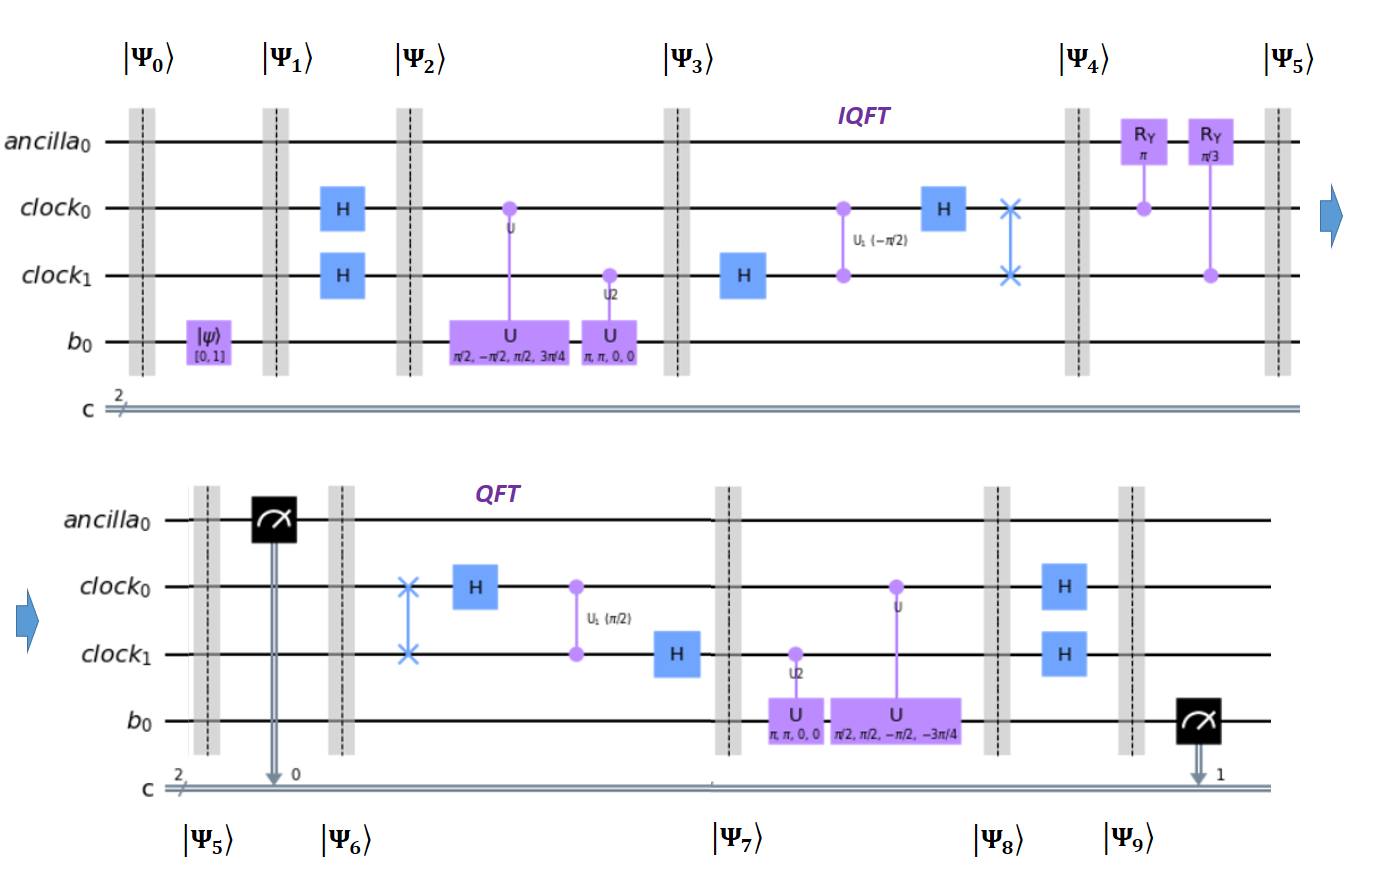
\includegraphics[width=0.7\textwidth]{/home/wangxinrui/Quantum-Computing/HHL3.png}
    \caption{本示例对应的HHL电路专为在IBM-Q上运行而构建,其划分方式与图1所示的通用HHL原理图相同。}
\end{figure}

\subsection{数值代入}

算法始于:
\[
|\Psi_0\rangle = |0\rangle_b \otimes |00\rangle_c \otimes |0\rangle_a = |0000\rangle
\]

施加X门(非门)将\(|0\rangle_b\)转换为\(|1\rangle_b\):
\[
|\Psi_1\rangle = X \otimes I \otimes I |\Psi_0\rangle = |1000\rangle
\]

对时钟量子比特施加Hadamard门产生叠加态:
\[
|\Psi_2\rangle = \frac{1}{2}(|1000\rangle + |1010\rangle + |1100\rangle + |1110\rangle)
\]

转换到\(A\)的特征向量基(因\(|1\rangle = \frac{1}{\sqrt{2}}(-|u_0\rangle + |u_1\rangle)\),故\(b_0 = \frac{-1}{\sqrt{2}}\)、\(b_1 = \frac{1}{\sqrt{2}}\)):
\[
\begin{aligned}
|\Psi_2\rangle &= \frac{1}{2\sqrt{2}}\left( -\left(|u_0\rangle|000\rangle + |u_0\rangle|010\rangle + |u_0\rangle|100\rangle + |u_0\rangle|110\rangle\right) + \right. \\
&\quad \left. \phantom{-\left( \right)} |u_1\rangle|000\rangle + |u_1\rangle|010\rangle + |u_1\rangle|100\rangle + |u_1\rangle|110\rangle \right)
\end{aligned}
\]

在受控旋转操作中,当对应时钟寄存器(c-register)处于状态\(|k\rangle_c\)时,需为本征向量\(|u_j\rangle\)添加相位变化\(\phi_j = \frac{k\lambda_j t}{2\pi}\)(即乘以相位因子\(e^{2\pi i\phi_j}\))。
代入\(t = \frac{3\pi}{4}\)、\(\lambda_0 = \frac{2}{3}\)、\(\lambda_1 = \frac{4}{3}\):
\[
\begin{aligned}
|\Psi_3\rangle &= \frac{1}{2\sqrt{2}} \left( -|u_{0}000\rangle - e^{2\pi i\phi_0}|u_{0}010\rangle - e^{2\pi i2\phi_0}|u_{0}100\rangle - e^{2\pi i3\phi_0}|u_{0}110\rangle \right. \\
&\quad \left. + |u_{1}000\rangle + e^{2\pi i\phi_1}|u_{1}010\rangle + e^{2\pi i2\phi_1}|u_{1}100\rangle + e^{2\pi i3\phi_1}|u_{1}110\rangle \right) \\
&= \frac{1}{2\sqrt{2}} \left( -|u_{0}000\rangle - e^{i\lambda_0 t}|u_{0}010\rangle - e^{i2\lambda_0 t}|u_{0}100\rangle - e^{i3\lambda_0 t}|u_{0}110\rangle \right. \\
&\quad \left. + |u_{1}000\rangle + e^{i\lambda_1 t}|u_{1}010\rangle + e^{i2\lambda_1 t}|u_{1}100\rangle + e^{i3\lambda_1 t}|u_{1}110\rangle \right) \\
&= \frac{1}{2\sqrt{2}} \left( -|u_{0}000\rangle - e^{i\pi/2}|u_{0}010\rangle - e^{i\pi}|u_{0}100\rangle - e^{i3\pi/2}|u_{0}110\rangle \right. \\
&\quad \left. + |u_{1}000\rangle + e^{i\pi}|u_{1}010\rangle + e^{i2\pi}|u_{1}100\rangle + e^{i3\pi}|u_{1}110\rangle \right) \\
&= \frac{1}{2\sqrt{2}} \left( -|u_{0}000\rangle - i|u_{0}010\rangle + |u_{0}100\rangle + i|u_{0}110\rangle \right. \\
&\quad \left. + |u_{1}000\rangle - |u_{1}010\rangle + |u_{1}100\rangle - |u_{1}110\rangle \right)
\end{aligned}
\]

在应用逆量子傅里叶变换(IQFT)之前,为简化计算,先对\(|\Psi_3\rangle\)的项进行重组,结果如下:
\[
|\Psi_3\rangle = \frac{1}{2\sqrt{2}} \left( \left(-|u_0\rangle + |u_1\rangle\right)|00\rangle + \left(-i|u_0\rangle - |u_1\rangle\right)|01\rangle + \left(|u_0\rangle + |u_1\rangle\right)|10\rangle + \left(i|u_0\rangle - |u_1\rangle\right)|11\rangle \right)|0\rangle
\]

接下来,对时钟寄存器(c-register)的量子态应用IQFT。以\(|10\rangle\)为例(其对应十进制数值为2),计算过程如下:
\[
\begin{aligned}
IQFT|10\rangle &= IQFT|2\rangle \\
&= \frac{1}{2^{2/2}} \sum_{y=0}^{2^2 - 1} e^{-2\pi i \cdot 2y / 4} |y\rangle \\
&= \frac{1}{2} \left(|0\rangle - |1\rangle + |2\rangle - |3\rangle\right) \\
&= \frac{1}{2} \left(|00\rangle - |01\rangle + |10\rangle - |11\rangle\right)
\end{aligned}
\]

同理,时钟寄存器其他基态经过IQFT后的结果为:
\[
IQFT|00\rangle = \frac{1}{2} \left(|00\rangle + |01\rangle + |10\rangle + |11\rangle\right)
\]
\[
IQFT|01\rangle = \frac{1}{2} \left(|00\rangle - i|01\rangle - |10\rangle + i|11\rangle\right)
\]
\[
IQFT|11\rangle = \frac{1}{2} \left(|00\rangle + i|01\rangle - |10\rangle - i|11\rangle\right)
\]

因此,将IQFT应用于\(|\Psi_3\rangle\),并代入上式,可得:
\[
\begin{aligned}
|\Psi_4\rangle &= IQFT|\Psi_3\rangle \\
&= \frac{1}{4\sqrt{2}} \Bigg( \left(-|u_0\rangle + |u_1\rangle\right)\left(|00\rangle + |01\rangle + |10\rangle + |11\rangle\right) + \\
&\quad \left(-i|u_0\rangle - |u_1\rangle\right)\left(|00\rangle - i|01\rangle - |10\rangle + i|11\rangle\right) + \\
&\quad \left(|u_0\rangle + |u_1\rangle\right)\left(|00\rangle - |01\rangle + |10\rangle - |11\rangle\right) + \\
&\quad \left(i|u_0\rangle - |u_1\rangle\right)\left(|00\rangle + i|01\rangle - |10\rangle - i|11\rangle\right) \Bigg)|0\rangle \\
&= \frac{1}{\sqrt{2}} \left(-|u_0\rangle|01\rangle + |u_1\rangle|10\rangle\right)|0\rangle
\end{aligned}
\]

可以看出,经过IQFT后,由于相长干涉,矩阵\(A\)的特征值仅在时钟寄存器处于\(|01\rangle\)和\(|10\rangle\)时具有非零振幅,即特征值被编码到时钟寄存器中。其中,\(\vec{b}\)在\(A\)本征向量基下的系数为\(b_0 = \frac{-1}{\sqrt{2}}\)、\(b_1 = \frac{1}{\sqrt{2}}\),且能清晰观察到b寄存器与c寄存器之间的纠缠关系---\(|u_0\rangle\)与\(|01\rangle\)关联,\(|u_1\rangle\)与\(|10\rangle\)关联。

在执行辅助量子比特旋转操作后,量子态表示为:
\[
\begin{aligned}
|\Psi_5\rangle &= \sum_{j=0}^{2^1 - 1} b_j \, |u_j\rangle \, |\tilde{\lambda}_j\rangle \left( \sqrt{1 - \frac{C^2}{\tilde{\lambda}_j^2}} \, |0\rangle + \frac{C}{\tilde{\lambda}_j} \, |1\rangle \right) \\
&= -\frac{1}{\sqrt{2}} \, |u_0\rangle \, |01\rangle \left( \sqrt{1 - \frac{1}{1^2}} \, |0\rangle + \frac{1}{1} \, |1\rangle \right) + \\
&\quad \frac{1}{\sqrt{2}} \, |u_1\rangle \, |10\rangle \left( \sqrt{1 - \frac{1}{2^2}} \, |0\rangle + \frac{1}{2} \, |1\rangle \right)
\end{aligned}
\]

若辅助比特测量结果为\(|1\rangle\):
\[
|\Psi_6\rangle = \sqrt{\frac{8}{5}}\left(-\frac{1}{\sqrt{2}}|u_0\rangle|01\rangle|1\rangle + \frac{1}{2\sqrt{2}}|u_1\rangle|10\rangle|1\rangle\right)
\]

将QFT应用于编码的特征值,我们得到

\[
\begin{aligned}
\text{QFT}|10\rangle &= \text{QFT}|2\rangle \\
&= \frac{1}{2^{2/2}} \sum_{y=0}^{2^2 - 1} e^{2\pi i \cdot 2y / 4} |y\rangle \\
&= \frac{1}{2} \bigl( |00\rangle - |01\rangle + |10\rangle - |11\rangle \bigr)
\end{aligned}
\]
% QFT作用于|01⟩的推导
\[
\begin{aligned}
\text{QFT}|01\rangle &= \text{QFT}|1\rangle \\
&= \frac{1}{2} \bigl( |00\rangle + i|01\rangle - |10\rangle - i|11\rangle \bigr)
\end{aligned}
\]

因此,对\(\lvert \Psi_6 \rangle\)应用量子傅里叶变换(QFT),并代入上述公式,我们得到

\[
\begin{aligned}
|\Psi_7\rangle &= \sqrt{\frac{8}{5}} \Biggl( -\frac{1}{\sqrt{2}} |u_0\rangle \cdot \frac{1}{2} \bigl( |00\rangle + i|01\rangle - |10\rangle - i|11\rangle \bigr)|1\rangle + \\
&\quad \frac{1}{2\sqrt{2}} |u_1\rangle \cdot \frac{1}{2} \bigl( |00\rangle - |01\rangle + |10\rangle - |11\rangle \bigr)|1\rangle \Biggr)
\end{aligned}
\]

对于受控旋转,若$c_0 = 1$和$c_1 = 1$,则量子态分别乘以$\text{e}^{-\text{i}\lambda_j t}$和$\text{e}^{-\text{i}2\lambda_j t}$。  
已知$\text{e}^{-\text{i}\lambda_0 t} = -\text{i}$、$\text{e}^{-\text{i}2\lambda_0 t} = -1$、$\text{e}^{-\text{i}\lambda_1 t} = -1$、$\text{e}^{-\text{i}2\lambda_1 t} = 1$,且$\frac{N t}{2\pi} = \frac{3}{2}$,则量子态$|\Psi_8\rangle$可表示为:  

\[
\begin{aligned}
|\Psi_8\rangle &= \sqrt{\frac{8}{5}} \Bigg[ -\frac{1}{\sqrt{2}} |u_0\rangle \cdot \frac{1}{2} \left( |00\rangle + |01\rangle + |10\rangle + |11\rangle \right)|1\rangle \\
&\qquad + \frac{1}{2\sqrt{2}} |u_1\rangle \cdot \frac{1}{2} \left( |00\rangle + |01\rangle + |10\rangle + |11\rangle \right)|1\rangle \Bigg] \\
&= \frac{1}{2}\sqrt{\frac{8}{5}} \left( -\frac{1}{\sqrt{2}} |u_0\rangle + \frac{1}{2\sqrt{2}} |u_1\rangle \right) \left( |00\rangle + |01\rangle + |10\rangle + |11\rangle \right)|1\rangle \\
&= \frac{1}{2} \cdot \frac{2}{3} \sqrt{\frac{8}{5}} \left( -\frac{3}{2\sqrt{2}} |u_0\rangle + \frac{3}{4\sqrt{2}} |u_1\rangle \right) \left( |00\rangle + |01\rangle + |10\rangle + |11\rangle \right)|1\rangle
\end{aligned}
\]

最后,对时钟量子比特施加哈达玛门(Hadamard gate),我们有:

\begin{equation}
\ket{\Psi_9} = \frac{2}{3}\sqrt{\frac{8}{5}} \left( -\frac{1}{\frac{2}{3}\sqrt{2}} \ket{u_0} + \frac{1}{\frac{4}{3}\sqrt{2}} \ket{u_1} \right) \ket{00} \ket{1} \tag{63}
\end{equation}

可以验证,$\ket{\Psi_9}$ 是一个归一化向量,理应如此,因为HHL电路中的每一个操作都是幺正的(酉操作),会保持范数(模长)不变。

通过将 $\ket{u_0} = \frac{-1}{\sqrt{2}}\ket{0} + \frac{-1}{\sqrt{2}}\ket{1}$ 和 $\ket{u_1} = \frac{-1}{\sqrt{2}}\ket{0} + \frac{1}{\sqrt{2}}\ket{1}$ 代入式 ,可对其进行化简。化简后,我们得到:

\begin{equation}
\ket{\Psi_9} = \frac{1}{2}\sqrt{\frac{2}{5}} \left( \ket{0} + 3\ket{1} \right) \ket{00} \ket{1} \tag{64}
\end{equation}

对b寄存器(b-register)进行测量时,测得 $\ket{0}$ 和 $\ket{1}$ 的概率比为 $1:9$ ,与预期一致。
\subsection{H门作用于$|\Psi_8\rangle$生成$|\Psi_9\rangle$的具体过程}
\subsubsection{初始态$|\Psi_8\rangle$的表达式}
施加H门前的量子态$|\Psi_8\rangle$可表示为:
\[
|\Psi_8\rangle = 
\underbrace{\frac{2}{3}\sqrt{\frac{8}{5}} \left( -\frac{1}{\frac{2}{3}\sqrt{2}} |u_0\rangle + \frac{1}{\frac{4}{3}\sqrt{2}} |u_1\rangle \right)}_{\text{系统部分}} 
\otimes 
\underbrace{\left( |00\rangle + |01\rangle + |10\rangle + |11\rangle \right)}_{\text{时钟量子比特(2量子比特)}} 
\otimes 
\underbrace{|1\rangle}_{\text{辅助量子比特}}
\]

\subsubsection{H门对2量子比特系统的作用}
H门作用于时钟量子比特(2个量子比特),其操作通过张量积实现:
\[
H_{\text{总}} = H \otimes H = \frac{1}{\sqrt{2}}
\begin{pmatrix} 1 & 1 \\ 1 & -1 \end{pmatrix} 
\otimes 
\frac{1}{\sqrt{2}}
\begin{pmatrix} 1 & 1 \\ 1 & -1 \end{pmatrix} 
= \frac{1}{2}
\begin{pmatrix} 
1 & 1 & 1 & 1 \\ 
1 & -1 & 1 & -1 \\ 
1 & 1 & -1 & -1 \\ 
1 & -1 & -1 & 1 
\end{pmatrix}
\]

对时钟量子比特基态的作用为:
\begin{align*}
H_{\text{总}}|00\rangle &= \frac{|00\rangle + |01\rangle + |10\rangle + |11\rangle}{2} \\
H_{\text{总}}|01\rangle &= \frac{|00\rangle - |01\rangle + |10\rangle - |11\rangle}{2} \\
H_{\text{总}}|10\rangle &= \frac{|00\rangle + |01\rangle - |10\rangle - |11\rangle}{2} \\
H_{\text{总}}|11\rangle &= \frac{|00\rangle - |01\rangle - |10\rangle + |11\rangle}{2}
\end{align*}

\subsubsection{H门作用于$|\Psi_8\rangle$的时钟部分}
对$|\Psi_8\rangle$中的时钟量子比特施加$H_{\text{总}}$:
\begin{align*}
H_{\text{总}} \left( |00\rangle + |01\rangle + |10\rangle + |11\rangle \right) &= 
H_{\text{总}}|00\rangle + H_{\text{总}}|01\rangle + H_{\text{总}}|10\rangle + H_{\text{总}}|11\rangle \\
&= \frac{|00\rangle + |01\rangle + |10\rangle + |11\rangle}{2} + \frac{|00\rangle - |01\rangle + |10\rangle - |11\rangle}{2} \\
&\quad + \frac{|00\rangle + |01\rangle - |10\rangle - |11\rangle}{2} + \frac{|00\rangle - |01\rangle - |10\rangle + |11\rangle}{2} \\
&= 2|00\rangle \quad (\text{化简后})
\end{align*}

\subsubsection{最终态$|\Psi_9\rangle$的生成}
系统部分和辅助量子比特不受H门影响,结合上述结果得到:
\[
|\Psi_9\rangle = 
\frac{2}{3}\sqrt{\frac{8}{5}} \left( -\frac{1}{\frac{2}{3}\sqrt{2}} |u_0\rangle + \frac{1}{\frac{4}{3}\sqrt{2}} |u_1\rangle \right) 
\otimes 
|00\rangle 
\otimes 
|1\rangle
\]
\end{document}